\begin{figure}[!t]
\centering
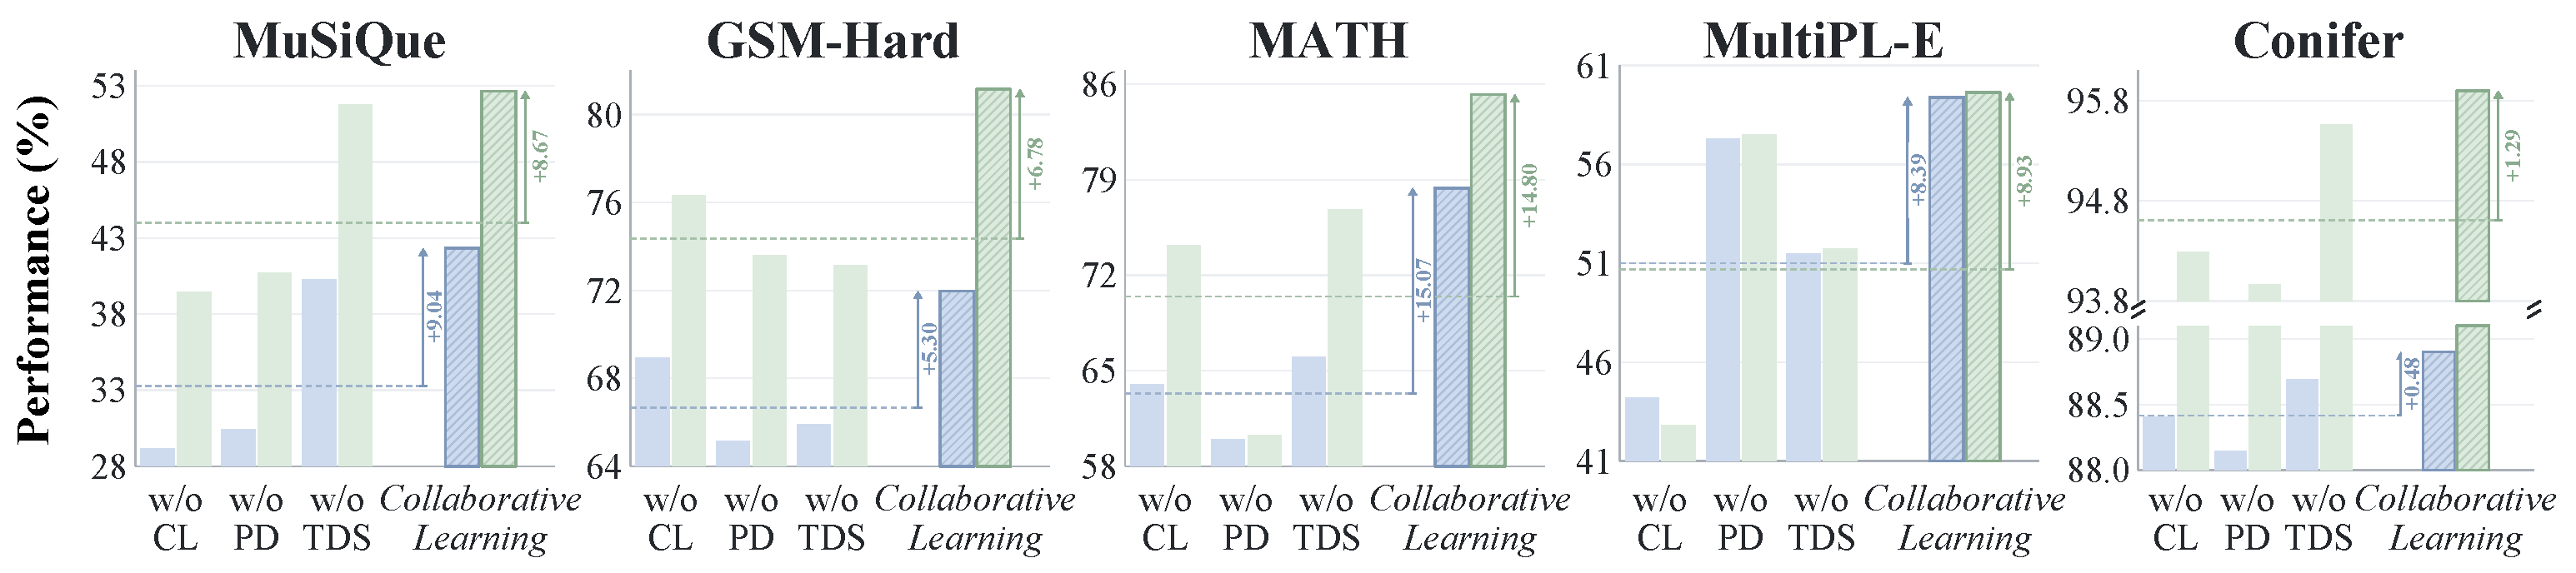
\includegraphics[width=\linewidth]{figures/Figure3.pdf}
\vspace{-1.5em}
\caption{\textbf{Ablation study of the mechanism across five benchmarks.} We compare variants without Protocol Distillation (PD) or the step-level deliberative score (TDS), together with a zero-shot variant that receives no training (w/o CL). Arrows indicate the gain of \textit{collaborative learning} over the arithmetic mean of the available variants. For each benchmark, \raisebox{0.15ex}{\textcolor[RGB]{206,219,239}{\rule{1.3em}{0.8em}}} denotes Acc., Wtd., and Cov., while \raisebox{0.15ex}{\textcolor[RGB]{220,235,221}{\rule{1.3em}{0.8em}}} denotes the corresponding second metric (F1, Mac., or Expl.).}
\label{fig:ablation_results}
\end{figure}